\Chapter{EMAIL2GIT: FROM ACADEMIC RESEARCH TO OPEN-SOURCE SOFTWARE}\label{sec:Theme2}


\section{Previous Publications and Original Algorithm}

The original algorithm capable of backtracking patches from commits was introduced in two papers~\citep{msr13jojo,jiang14} published by Jiang, a former member of the MCIS Lab. Originally written in Perl, the script was a great proof of concept. The general idea of the script was to compare the +/- lines from both the git commits and the email patches. A match was found if the proportion of identical +/- lines was above a certain threshold. Although this script was a great proof of concept, it had difficulties scalling to 8 years of emails and commits. 



\section{Scalling the Algorithm}

Because we wanted Email2git to be a usable and practical tool, we needed a way to display the patches and the code reviews in a browser. Fortunatly, a great existing open-source tool called \textbf{Patchwork}\footnote{\url{https://github.com/getpatchwork/patchwork}} perfectly answers our requirements. Patchwork is a tool designed to assist maintainers of open source projects using an email-based contribution process. It tracks the mailing lists used by developers to submit patches and recieve code reviews. The tool extracts each detected patch as well as its associated reviews, then displays them in a web-based user interface. 

We were granted read access to the MySQL database behind a patchwork instance hosted on kernel.org\footnote{\url{https://patchwork.kernel.org/}}. This instance has been tracking 69 of the many linux subsystems mailing lists since 2009, giving us the oportunity to analyse over \textit{1.4 million} patches.

In addition to being a great data source, patchwork.kernel.org is also a great way for us to display the patches and the code reviews associated with commits to the users. The only limitation of this patchwork instance is that it does not track some major mailing lists, particularly some of the \texttt{Net} mailing lists. 


Since we had access to email patches dating back to 2009, we decided to extract git commits from the Linux git repository from the same date, which represent over \textit{500,000 commits} to analyse. Unfortunatly, this amount of data was too large for the orignal algorithm to parse in a timely fashion, which called for a new, scalable algorithm that leverages heuristics mentioned in \citep{msr13jojo,jiang14}.

\subsection{Patch Email Subject}

The most important heuristic that drastically increased the matching speed is the \textit{email subject - commit summary} concept. The built-in git features \texttt{git format-patch} and \texttt{git send-email} allows developers to easily submit their changes to a maintainer by email according to the Linux Kernel Contribution guidelines\footnote{\url{https://kernelnewbies.org/FirstKernelPatch}}. This or these emails contain all the meta-data that will eventually be included in the commit, if the patch is accepted. The meta-data includes heuristics such as: time sent, author, commit message, ... If the patch is accepted, the maintainer can use another git command to integrate the patch into her repository: \texttt{git am}\footnote{\url{https://git-scm.com/docs/git-am}}. This command will automatically exctract the patch info and keep the relevant information in the commit. The piece of information we are interested in is the email subject. \texttt{Git am} automatically saves the email subject and uses it the "commit summary". This commit summary, or commit title, is the first line of the commit message (((TODO: refer to intro for git commit stuff))). Comparing both strings of characters allows for a very quick first phase of matching.

This first phase will find a match for about 55\% of the commits. After this step, we can remove the commits and the patches that were matches from the "search space", reducing the amount of patches and commits to be parsed, reducing the load on the algorithm. 

\subsection{Author and Affected Files}

Even though the number of commits was reduced by half, I was unable to make the old script fast enough to parse the rest of the data in a timely fashion. Thus, I had to find a new way to use the available meta-data to speed up the matching. The first data point I used was the \textit{author name}.  


\begin{figure}[htb]
\centering
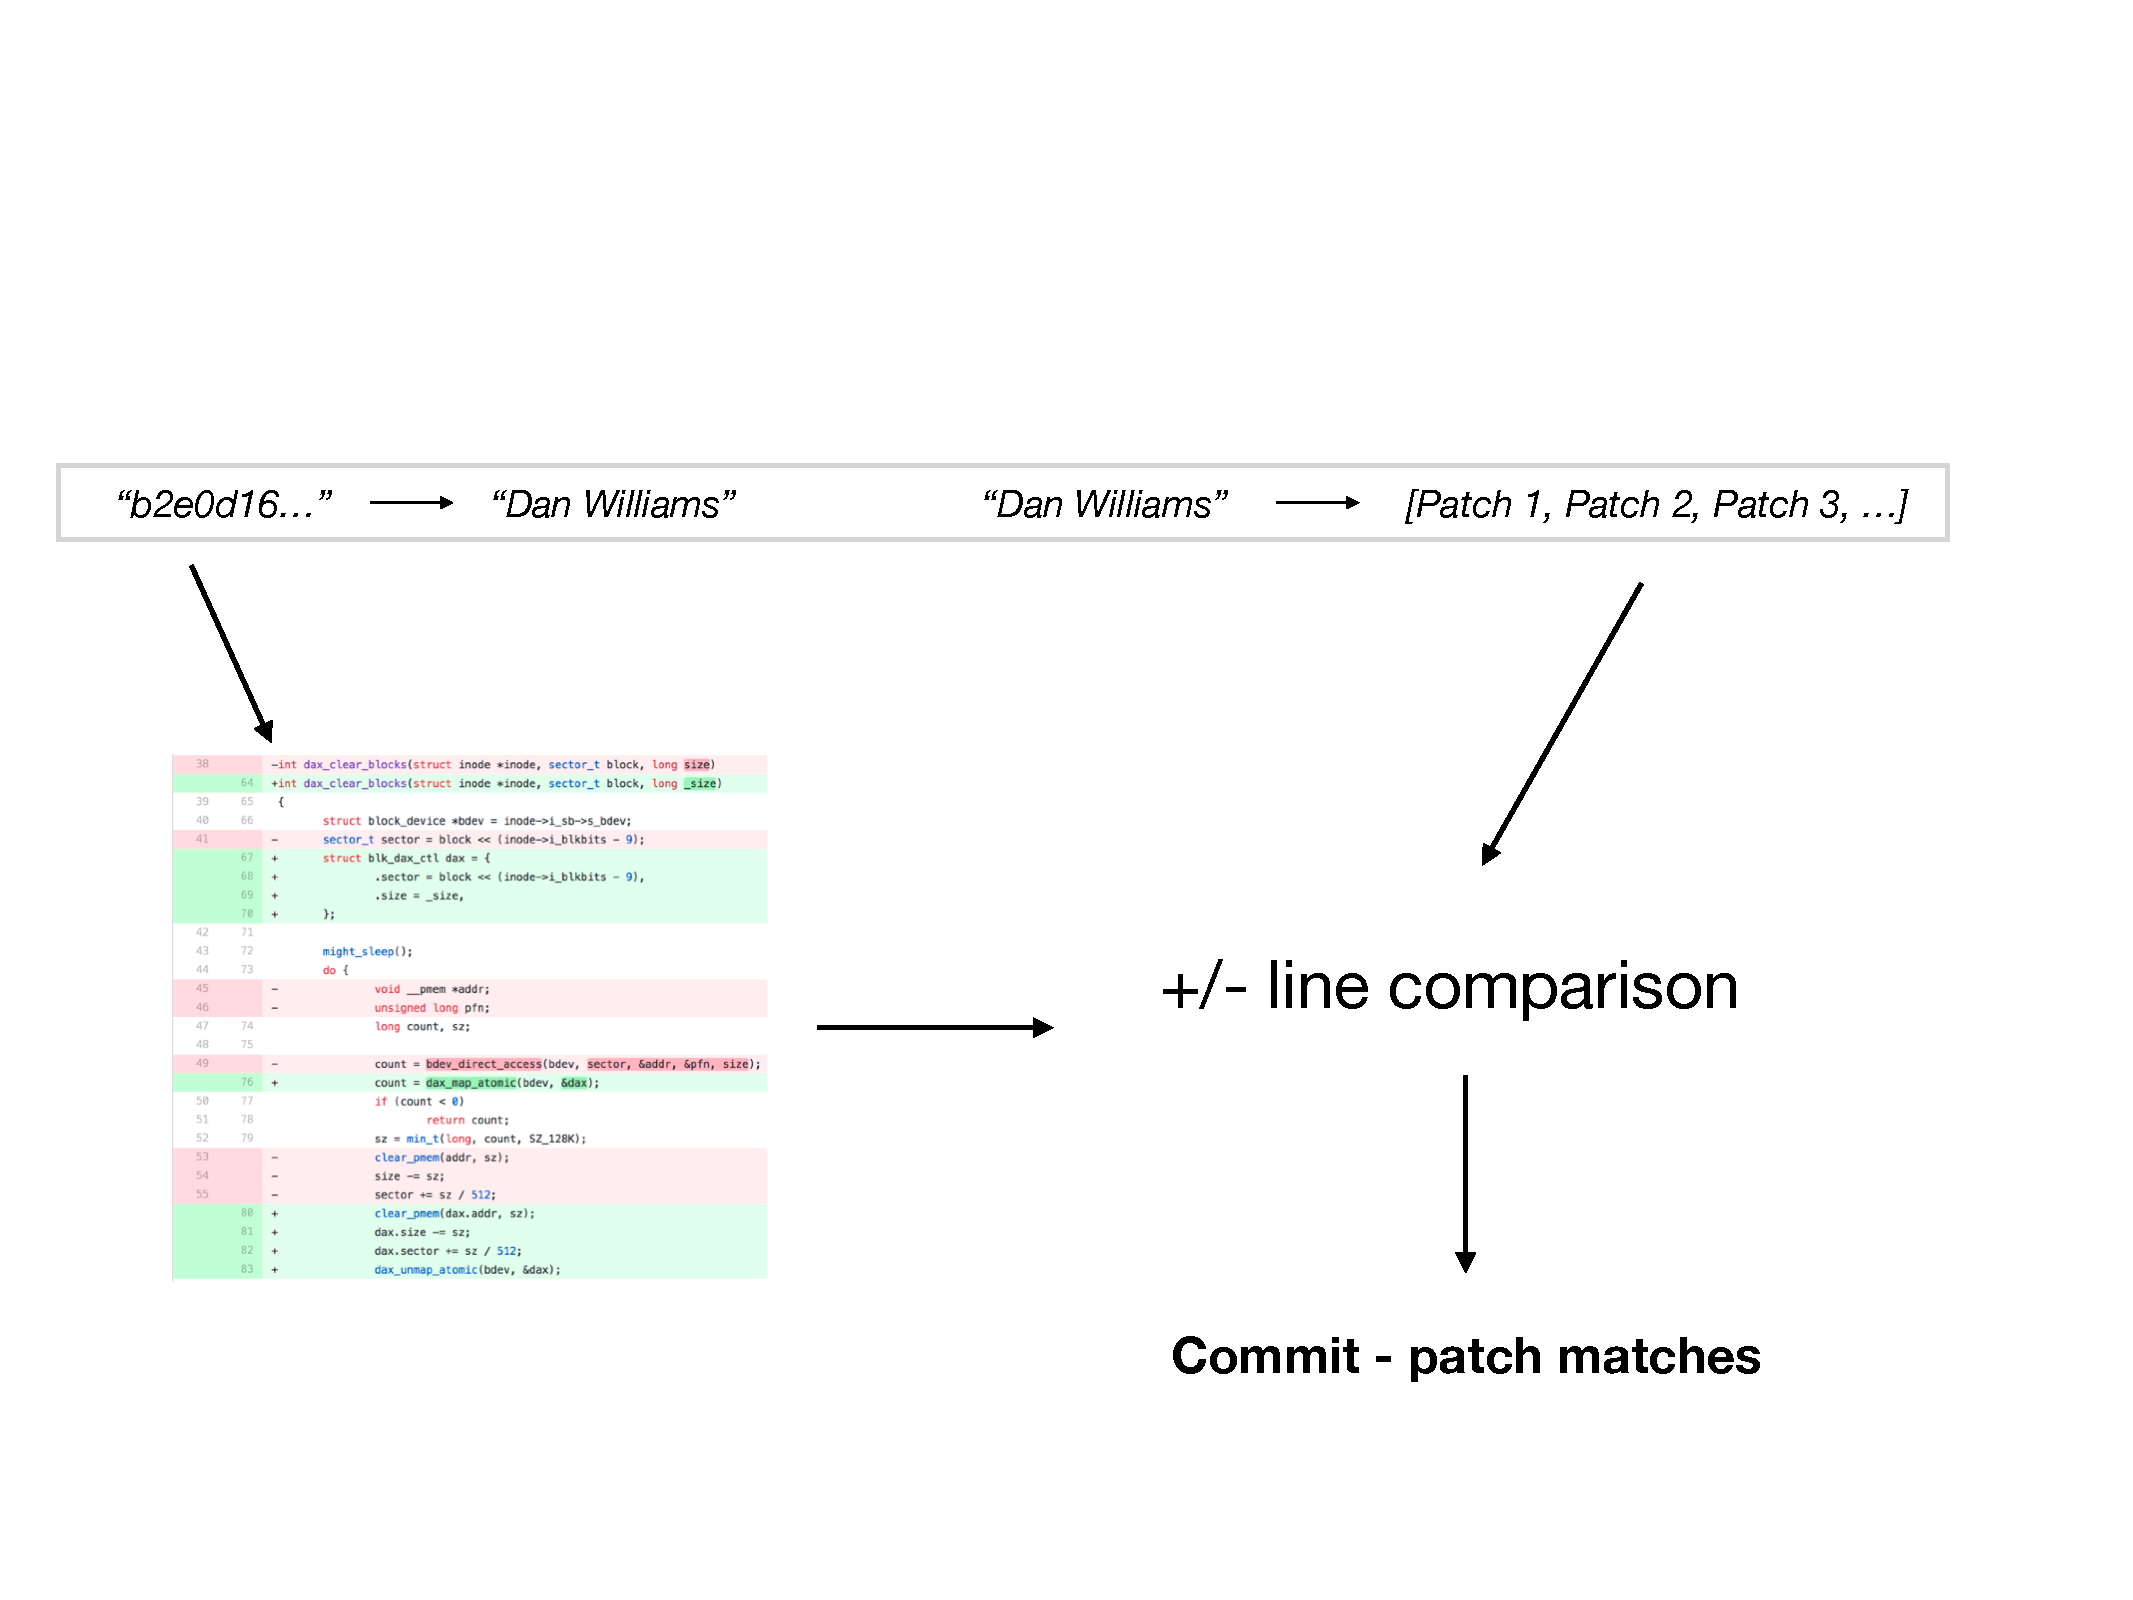
\includegraphics[width=5in]{author_matching}
\caption{Using the patch sender to assist matching}
\label{fig:author_matching}
\end{figure}


\section{The Data}

There are two sides to this matching process: the Linux git repository and the archives containing the patches sent in mailing lists over the years. We need to extract data from both sides. 

\subsection{Extracting the Commits}


\subsection{Extracting the Patches}








\section{Serving the Matches}





